% Cite:
% crp          (done)
% Radford Neal (done)
% Blei. ddcrp  (done)
% IBP          (done)
% Dahl. partition distribution including pairwise info
% Blei. ddIBP

% Topics: Talk about paper Here's what I am talking about, and pull the paper
% to show it's true

\chapter{Literature Review} % ~15 pages We will first review the Chinese
Before discussing how we will propose a new distribution, we will first review 
some familiar processes and distributions. We will discuss the Chinese restaurant 
process (CRP), the distance dependent Chinese restaurant process (ddcrp),
the Ewens-Pitman attraction (EPA) distribution, % Cite Dahl 
and the Indian buffet process (IBP).
%, and the distance dependent Indian buffet process (dd-IBP). 
%formulated by Gershman. % Cite Finally, we will finally review existing McMC
%methods for sampling from the IBP.  Maybe applications also?

\subsection{The Chinese Restaurant Process}
The Chinese restaurant process (CRP) describes the dirichlet process, a process
that creates partition distributions. The partition distribution generated by the 
CRP is the Ewens-Pitman distribution. The CRP can be described as follows.\\

\noindent
A number of customers (observations), n, enter a Chinese restaurant to be
seated one at a time. Let $z_i$ be the table (cluster) number that each
customer gets assigned to, such that $z_i \in \left\{ 1,..,n \right\}$, for
$i = 1,...,n$. Then,
\begin{equation}
  P(z_i=k|z_{1:(i-1)},\alpha) \propto 
  \begin{cases}
    \begin{array}{rll}
      n_k,    & \text{if} & k \le K\\
      \alpha, & \text{if} & k = K+1\\
    \end{array}
  \end{cases}
\end{equation}
where the normalizing constant is ${(\alpha+i-1)}^{-1}$, $n_k$ is the number
of customers in table k before seating customer $i$, K is the number of
occupied tables before seating customer $i$, and $\alpha$ is a mass parameter
which determines the number of tables that will eventually be occupied by the n
customers. The larger $\alpha$ is, the greater the final number of occupied
tables. The resulting partition distribution is called the Ewans-Pitman
distribution. And if we let $\pi_n$ represent the partition
$\left\{S_1,...,S_{q_n}\right\}$, where $q_n \in \lb1,...,n\rb$ and represents
the number of partitions, and each $S_i$ is a set representing a cluster or
customers seated at table $i$, $\pi_n$ will have the properties: (1) $S_i \cap
S_j = \o$ for $i \ne j$ (sets are mutually exclusive), (2) $\underset{S \in
\pi_n}{\cap} S = \lb 1,...,n \rb$ (sets are exhaustive), and (3) $S_i \ne \o$,
$\forall i \in \lb 1,...,q_n\rb$ (no sets are empty).  The probability mass
function for this partition distribution, the Ewens-Pitman distribution, is
\begin{equation}
  P(\pi_n) = \underset{S \in \pi_n}{\prod} 
             \frac{\alpha\Gamma(|S|)}{\alpha^{(n)}}
\end{equation}

\noindent
Gibbs samplers to generate this process have been studied extensively. 
A valuable list and comprison of algorithms to draw from the posterior with 
a CRP prior was compiled by Neal (2000). An implementation of some of these
algorithms in \textbf{R} and \textbf{SCALA} can be found at my github account: 
https://github.com/luiarthur/auxGibbs/tree/master/scala\\

%\noindent
%I will describe Algorithm 8 from Neals paper. \\
%Let the state


\subsection{Distance Dependent Chinese Restaurant Process}
Researchers such as Blei \& Frazier have extended CRP to include 
distance information. The distribution they have proposed is the distance
dependent Chinese restaurant process (ddCRP). \\

\noindent
Given a distance matrix, D, and a mass parameter, $\alpha$, the probability
of customer $i$ being ``assigned" to sit with customer $j$ is 
\begin{equation}
  P(c_i=j|D,\alpha) \propto 
  \begin{cases}
    \begin{array}{rll}
      f(d_{ij}), & \text{if} & j \ne i\\
      \alpha,    & \text{if} & i=j
    \end{array}  
  \end{cases}
\end{equation}
where $f(d_{ij})$ is a decay function with the properties: (1) $f(\cdot) \ge 0$,
(2) $f(\infty) = 0$, and $f(\cdot)$ is non-decreasing. The normalizing constant 
is again $(\alpha+i-1)^{-1}$. Customers assigned to sit together at a table
form a cluster. The resulting distribution is a partition distribution that
includes pairwise distance information. However, no closed form probability 
mass function for the resulting partition distribution has been written for 
Blei's proposed ddcrp. Blei describes a Gibbs sampler to sample from the 
ddcrp and its posterior.

\subsection{Ewens-Pittman Attraction Distribution}
The Ewens-Pitmann Attraction (EPA) distribution is another partition
distribution that incorporates pairwise distance information. Before
introducing the probability mass function, I will review some notation.\\

\noindent
Let $\pi_n$ be a discrete partition distribution, as defined in the previous
section. Let the permutation $\bm \sigma = (\sigma_1,...,\sigma_n)$ be the order
in which each item is allocated, where the $t^{th}$ item to be allocated is
$\sigma_t$. This is not necessarily the order of the n items in the dataset. In
addition, at time $t > 1$, let $\pi(\sigma_{1},...,\sigma_{t-1})$ represent the
current partition created from allocating $\sigma_{1},...,\sigma_{t-1}$. Note
that the complete partition $\pi_n = \pi(\sigma_{1},...,\sigma_{n})$.\\

\noindent
The EPA distribution incorporates pairwise distance information. A possible
metric for measuring distance is the Euclidean metric. Let $d_{ij}$ denote the
distance between two items, $i$ and $j$. Let the function $\lambda(i,j)$ represent
the similarity of items $i$ and $j$ (i.e. how ``close" two items are, where a larger
value indicates that the two items are closer together). A large class of similarity
functions can be represented as a function of the distance information. That is
$\lambda(i,j)$ can be written as $f(d_{ij})$ in many cases, where $f(\cdot)$ is a
non-increasing function. For instance, $\lambda(i,j)$ can be ${d_{ij}}^{-\tau}$,
where $\tau>0$ and is called the \textit{temperature} and can dampen or
accentuate the effect of distance.\\

\noindent
The EPA distribution is also defined by a mass parameter, $\alpha > 0$, and a discount
parameter, $\delta \in [0,1)$. The probability mass function for a partition 
distribution $\pi_n$ following the EPA distribution can be defined as follows:
\begin{equation}
  p(\pi_n|\alpha,\delta,\lambda,\bm\sigma)=
    \prodl{i}{1}{n}p_t(\alpha,\delta,\lambda,\pi(\sigma_1,...,\sigma_{t-1}))
\end{equation}
where $p_t(\alpha,\delta,\lambda,\pi(\sigma_1,...,\sigma_{t-1}))$ is defined as:
\begin{equation}
  P(\sigma \in S | \alpha,\delta,\lambda,\pi(\sigma_1,...,\sigma_{t-1}))=
  \begin{cases}
    \begin{array}{ll}
      \ds\frac{t-1-\delta q_{t-1}}{\alpha+t-1} \cdot 
        \frac{\sum_{\sigma_s \in S}\lambda(\sigma_t,\sigma_s)}
        {\sum_{s=1}^{t-1}\lambda(\sigma_t,\sigma_s)} & 
        \text{for }S \in \pi(\sigma_1,...,\sigma_{t-1})\\
      \ds\frac{\alpha+\delta q_{t-1}}{\alpha+t-1} &  \text{for }S  = \o \\
    \end{array}
  \end{cases}
\end{equation}
Note that the ratio of sums in (2.5) represents the proportion of \textit{total
attraction} of item $\sigma_t$ to the items allocated to subset $S$.



\noindent
\textbf{STOPPED RIGHT HERE!!!}
%%%%%TALK ABOUT THE PARTITION NOTATION!!!
%%%%%TALK ABOUT THE PARTITION NOTATION!!!
%%%%%TALK ABOUT THE PARTITION NOTATION!!!
%%%%%TALK ABOUT THE PARTITION NOTATION!!!



\subsection{The Indian buffet process}
One key problem in recovering the latent structure responsible for generating
observed data is determining the number of latent features. The Indian Buffet
process (IBP) provides a flexible distribution for sparse binary matrices with
infinite dimensions (i.e. finite number of rows, and infinite number of columns).
When used as a prior distribution in a latent feature model, the IBP can
learn the number of latent features generating the observations because it can
draw binary matrices which have a potentially infinite number of columns. I will
use the IBP as a prior distribution in a Gaussian latent feature model to
recover the latent structures generating the observations.\\

\noindent
The IBP is a distribution for sparse binary matrices with finite number of rows
and potentially infinite number of columns. The process of generating a
realization from the IBP can be described by an analogy involving Indian buffet
restaurants.\\

\noindent
Let $Z$ be an $N \times \infty$ binary matrix. Each row in $Z$ represents a
customer which enters an Indian buffet and each column represents a dish in the
buffet. Customers enter the restaurant one after another. The first customer
samples an $r=$Poisson$(\alpha)$ number of dishes, where $\alpha > 0$ is a mass
parameter which influences the final number of sampled dishes. This is
indicated in by setting the first r columns of the first row in $Z$ to be $1$.
The other values in the row are set to $0$. Each subsequent customer samples
each previously sampled dish with probability proportional to its popularity.
That is, the next customer samples dish $k$ with probability $\frac{m_k}{i}$,
where $m_k$ is the number of customers that sampled dish $k$, and $i$ is the
current customer number (or row number in $Z$). Each customer also samples an
additional Poisson$(\alpha/i)$ number of new dishes. Once all the $N$ customers
have gone through this process, the resulting $Z$ matrix will be a draw from
the Indian buffet process with mass parameter $\alpha$. In other words, $Z \sim
\text{IBP}(\alpha)$. Note that $\alpha \propto K_+$, where $K_+$ is the final number of
sampled dishes (occupied columns). Figure 2.1 shows a draw from an IBP(10) with 50
rows. The white squares are 1, indicating that a dish was taken; black squares
are 0, indicating that a dish was not taken. \\
\beginmyfig
  \caption{IBP($N=50$, $\alpha=10$)}
  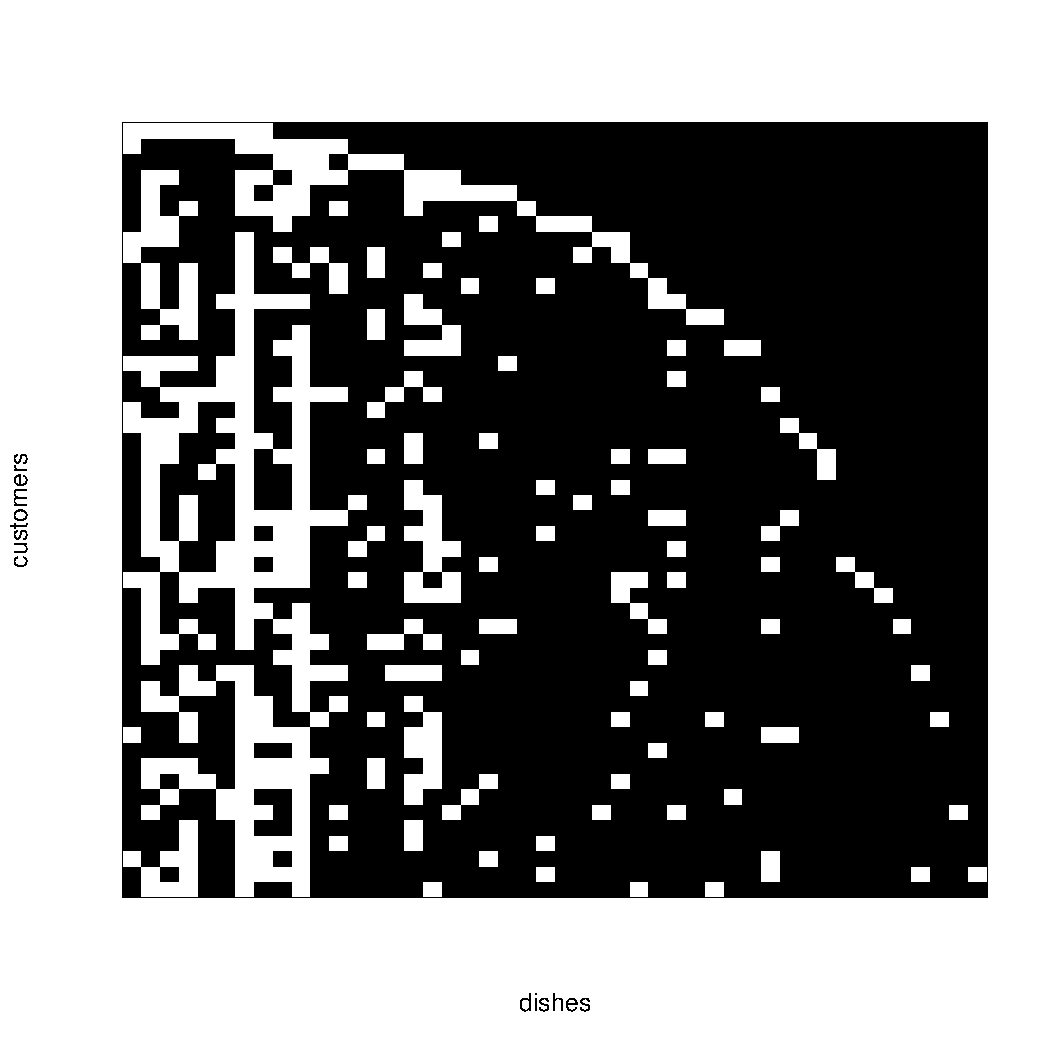
\includegraphics{images/ibp.pdf}
\endmyfig

\noindent
The probability of any particular matrix produced from this process is
\begin{equation}
  P(\bm{Z}) = \frac{\alpha^{K_+}}{\prodl{i}{1}{N} {K_1}^{(i)}!} 
              exp\{-\alpha H_N\}\prodl{k}{1}{K_+}
              \frac{(N-m_k)!(m_k-1)!}{N!},
\end{equation}
where $H_N$ is the harmonic number, $\suml{i}{1}{N}\ds\frac{1}{i}$, $K_+$ is
the number of non-zero columns in $\bm Z$, $m_k$ is the $k^{th}$ column sum of
$\bm Z$, and $K_1^{(i)}$ is the ``number of new dishes" sampled by customer $i$.\\

\noindent
One way to get a draw from the IBP($\alpha$) is to simulate the process according to 
the description above. Another way is to implement a Gibbs sampler as follows:

\begin{enumerate}
  \item Start with an arbitrary binary matrix of $N$ rows
  \item For each row, $i$,
  \begin{enumerate}
    \item For each column, $k$,
    \item if $m_{-i,k}$ = $0$, delete column $k$. Otherwise,
    \item set $z_{ik}$ to $0$
    \item set $z_{ik}$ to $1$ with probability $P(z_{ik}=1|\bm{z_{-i,k}}) = \frac{m_{-i,k}}{i}$
    \item at the end of row $i$, add Poisson($\ds\frac{\alpha}{N}$) columns of $1$'s
  \end{enumerate}
  \item iterate step 2 a large number of times
\end{enumerate}
We can likewise incorporate this Gibbs sampler to sample from the posterior distribution P($\bm{Z|X}$)
where $\bm Z \sim \text{IBP}(\alpha)$ by sampling from the complete conditional
\begin{equation}
  P(z_{ik}=1|\bm{Z_{-(ik)},X})  \propto p(\bm{X|Z}) P(z_{ik}=1|\bm{Z_{-(ik)}}).
\end{equation}\\


\noindent
Note that a conjugate prior for $\alpha$ is a Gamma distribution.
\[
  \begin{array}{rcl}
    \bm Z|\alpha & \sim & \text{IBP}(\alpha)\\
          \alpha & \sim & \text{Gamma}(a,b), \text{where $b$ is the scale parameter}\\
    & & \\
    p(\alpha|\bm Z) & \propto & p(\bm Z|\alpha) p(\alpha)\\
    p(\alpha|\bm Z) & \propto & \alpha^{K_+} e^{-\alpha H_N}  
                                \alpha^{a-1} e^{-\alpha/b}\\
    p(\alpha|\bm Z) & \propto & \alpha^{a+K_+-1} e^{-\alpha(1/b+H_N)}\\
  \end{array}
\]
\begin{equation}
  \alpha|\bm Z  \sim  \text{Gamma}(a+K_+, (1/b+H_N)^{-1})
\end{equation}

% IBP Implementation.

%\subsection{Distance Dependent Indian Buffet Process}
%Currently, there exists a distance dependent Indian buffet process (dd-IBP), 
%constructed by Gershman, Frazier, and Blei (2012). We wish to create a model 
%similar to it. We will first review the ddIBP.





%The applications of the Indian buffet distribution include defining priors

% What is the IBP? # Done
% Gibbs sampler to draw from prior # Done
% Gibbs sampler to draw from posterior # Done
% What is it used for?
% Where are the applications?
% Why would it be useful to include distance information?
% ddIBP?

